\subsection{Interaction forte}\label{chapter-MS-MSSM-section-formalisme-subsec-QCD}
\subsubsection{La couleur}\label{chapter-MS-MSSM-section-formalisme-subsec-QCD-subsubsec-couleur}
L'interaction forte est la troisième force fondamentale décrite par le modèle standard.
L'analogue de la charge électrique pour l'interaction électromagnétique est, dans le cas de l'interaction forte, la \og couleur \fg,
concept né de l'observation des baryons \Deltabaryonplusplus, \Deltabaryonminus, \Omegabaryonminus.
Dans le modèle des quarks, ces baryons sont composés comme
\begin{equation}
\Deltabaryonplusplus = (\quarku\quarku\quarku)
\msep
\Deltabaryonminus = (\quarkd\quarkd\quarkd)
\msep
\Omegabaryonminus = (\quarks\quarks\quarks)
\mend
\end{equation}
Or, ces baryons sont de spin $\frac{3}{2}$. Les quarks possédant un spin $\frac{1}{2}$, il faudrait alors que pour chacun de ces baryons, les trois quarks les composant aient leurs nombres quantiques égaux, ce qui va à l'encontre du principe de Pauli.
\par En introduisant la charge de couleur, pouvant prendre trois valeurs orthogonales que l'on nomme par convention rouge, vert et bleu, il est possible de décrire ces baryons sans violer le principe d'exclusion de Pauli. Il suffit en effet que chaque quark porte une couleur différente, \ie
\begin{equation}
\Deltabaryonplusplus = ({\color{red}\quarku}{\color{green}\quarku}{\color{blue}\quarku})
\msep
\Deltabaryonminus = ({\color{red}\quarkd}{\color{green}\quarkd}{\color{blue}\quarkd})
\msep
\Omegabaryonminus = ({\color{red}\quarks}{\color{green}\quarks}{\color{blue}\quarks})
\mend
\end{equation}
\par Les baryons ainsi formés de trois quarks (un rouge, un vert et un bleu) portent une charge de couleur globale nulle, ils sont de couleur \og blanche \fg. Il en va de même pour les mésons, formés d'un quark un d'un anti-quark. Les anti-quarks portent une \og anti-couleur \fg, ainsi l'association d'un quark d'une couleur avec un anti-quark de l'anti-couleur correspondante donne un méson \og blanc \fg. La neutralité de couleur des hadrons (baryons et mésons) est effectivement confirmée expérimentalement et résulte du phénomène de \og confinement de couleur \fg, abordé dans la section~\ref{chapter-MS-MSSM-section-formalisme-subsec-QCD-subsubsec-confinement}.
\subsubsection{Symétrie $SU(3)_C$}\label{chapter-MS-MSSM-section-formalisme-subsec-QCD-subsubsec-SU3C}
Afin de décrire l'interaction forte dans le même formalisme que les autre interactions fondamentales, il nous faut un groupe de symétrie. Étant donné qu'il existe trois dimensions de couleur (rouge, verte, bleue), la théorie quantique des champs associée à l'interaction forte se base sur le groupe $SU(3)_C$, où $C$ signifie \og couleur \fg.
\par Tout comme $SU(2)$, $SU(3)$ est un groupe non abélien. Il est possible de reprendre exactement les mêmes calculs que ceux de la section~\ref{chapter-MS-MSSM-section-formalisme-subsec-EW-SU2_general}, en procédant aux changements\footnote{La constante de couplage pour l'interaction forte est souvent notée $\alpha_s$. Nous utilisons ici la notation $g_s$ afin d'illustrer le rôle analogue avec celui $g_Y$ et $g_I$.}
\begin{equation}
\bm{\tau} \in \mathcal{M}_2(\mathbb{C})^3 \leftrightarrow \bm{\lambda} \in \mathcal{M}_3(\mathbb{C})^8
\msep
\bm{\alpha}\in\mathbb{R}^3 \leftrightarrow \bm{\theta}\in\mathbb{R}^8
\msep
g_I \leftrightarrow g_s
\msep
\bm{W}_\mu \leftrightarrow \bm{G}_\mu
\msep
\bm{W}_{\mu\nu} \leftrightarrow \bm{G}_{\mu\nu}
\label{eq-hapter-MS-MSSM-section-formalisme-subsec-QCD-subsubsec-SU3C-analogieSU2}
\end{equation}
où $\bm{\lambda}$ est un vecteur à huit composantes, chacune étant une matrice de Gell-Mann, définies dans l'annexe~\ifref{annexe-maths}{\ref{annexe-maths}}{A} et où $\bm{G}_\mu$ décrit donc huit gluons, bosons vecteurs de l'interaction forte.
\par Le terme non linéaire $\bm{G}_\mu\wedge\bm{G}_\nu$ dans l'expression de $\bm{G}_{\mu\nu}$\footnote{Obtenue à partir de l'analogie~\eqref{eq-hapter-MS-MSSM-section-formalisme-subsec-QCD-subsubsec-SU3C-analogieSU2} appliquée à l'équation~\eqref{eq-chapter-MS-MSSM-section-formalisme-subsec-EW-defWmunu}.} est lourd de conséquences.
Il permet le couplage entre trois et quatre gluons, comme cela est illustré sur la figure~\ref{fig-fgraph-QCD_3_et_4_gluons}, et donne à l'interaction forte toute sa singularité. En effet, ce terme est responsable de l'initiation de la gerbe partonique qui donne naissance aux jets, dont il est question au chapitre~\ifref{chapter-JERC}{\ref{chapter-JERC}}{sur la calibration en énergie des jets}, ainsi que du confinement de couleur.
\begin{figure}[h]
\centering
\vspace{\baselineskip}
\subcaptionbox{\label{subfig-fgraph-ggg}}[.45\textwidth]
{\begin{fmffile}{ggg}\fmfstraight
\begin{fmfchar*}(20,20)
  \fmfleft{i1}
  \fmfright{o1,o2}
  \fmf{gluon}{i1,v}
  \fmf{gluon}{o1,v}
  \fmf{gluon}{o2,v}
  \fmfdot{v}
  \fmflabel{\gluon}{i1}
  \fmflabel{\gluon}{o1}
  \fmflabel{\gluon}{o2}
\end{fmfchar*}
\end{fmffile}\vspace{\baselineskip}}
\hfill
\subcaptionbox{\label{subfig-fgraph-gggg}}[.45\textwidth]
{\begin{fmffile}{gggg}\fmfstraight
\begin{fmfchar*}(20,20)
  \fmfleft{i1,i2}
  \fmfright{o1,o2}
  \fmf{gluon}{i1,v}
  \fmf{gluon}{i2,v}
  \fmf{gluon}{o1,v}
  \fmf{gluon}{o2,v}
  \fmfdot{v}
  \fmflabel{\gluon}{i1}
  \fmflabel{\gluon}{i2}
  \fmflabel{\gluon}{o1}
  \fmflabel{\gluon}{o2}
\end{fmfchar*}
\end{fmffile}\vspace{\baselineskip}}

\caption{Diagrammes de Feynman correspondant à l'interaction entre trois et quatre gluons.}
\label{fig-fgraph-QCD_3_et_4_gluons}
\end{figure}
\subsubsection{Confinement de couleur}\label{chapter-MS-MSSM-section-formalisme-subsec-QCD-subsubsec-confinement}

\begin{equation}
g_s (k) = \frac{6\pi}{(33-2n_f)\ln(\frac{k}{\Lambda_\text{QCD}})}
\msep
\Lambda_\text{QCD} = 218\pm\SI{24}{\MeV}
\mend
\end{equation}
avec $n_f$ le nombre de saveurs de quarks (6, ou plutôt le nombre de générations = 3 ?), $\Lambda_\text{QCD}$ l'échelle d'énergie à laquelle $g_s$ diverge.
%the coupling decreases logarithmically, a phenomenon known as asymptotic freedom (the discovery of which was awarded with the Nobel Prize in Physics in 2004).

\begin{figure}
\centering
\begin{tikzpicture}
\node[anchor=south west,inner sep=0] at (0,0) {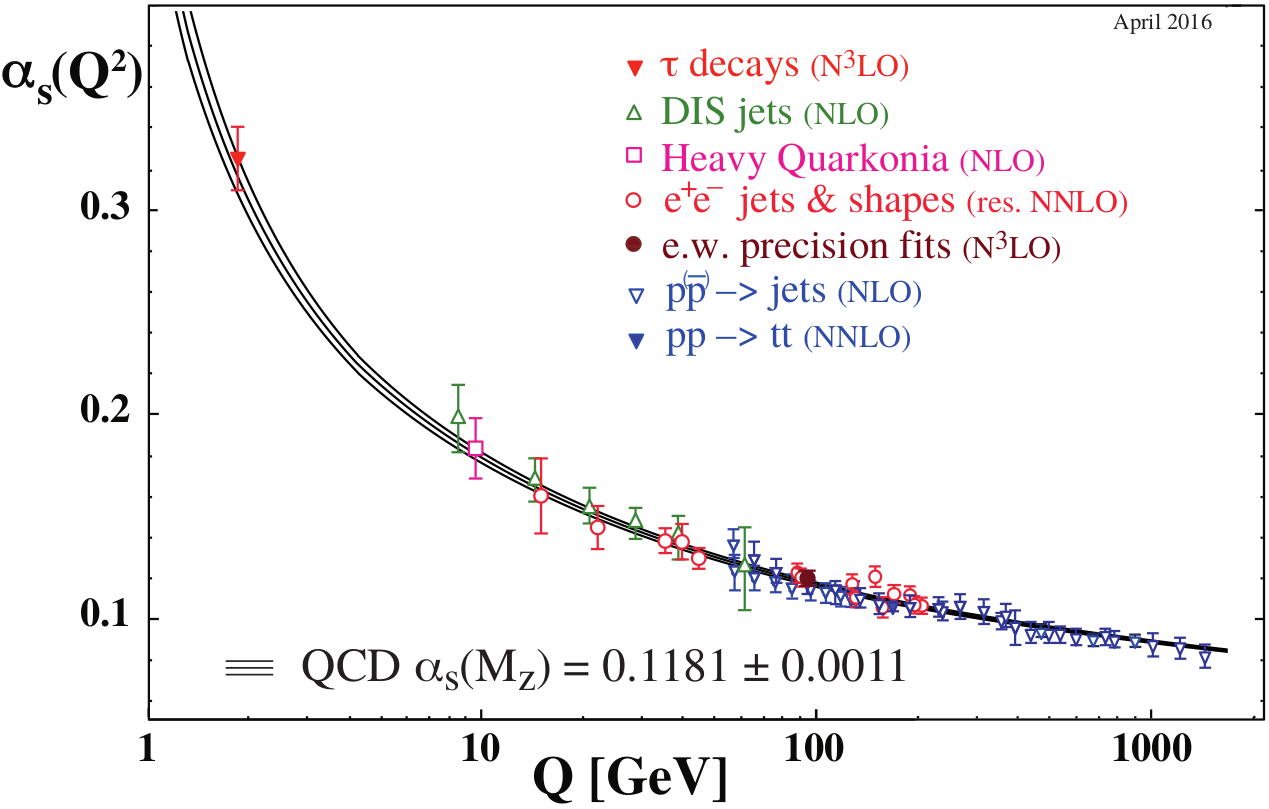
\includegraphics[width=10cm]{\PhDthesisdir/contents/chapter-MS-MSSM/formalisme/QCD_value_fct_Q.png}};
\fill [white] (1,0) rectangle (10, .65);
\fill [white] (1.15,0) rectangle (0,6);
\fill [white] (1.5,.85) rectangle (7.2,1.3);

\draw (1.2,.5) node {\small \num{1}} ;
\draw (3.8,.5) node {\small \num{10}} ;
\draw (6.45,.5) node {\small \num{100}} ;
\draw (9.1,.5) node {\small \num{1000}} ;

\draw (5,.25) node {$k$ (\SI{}{\GeV})} ;

\draw (.8,1.5) node {\small \num{0.1}} ;
\draw (.8,3.15) node {\small \num{0.2}} ;
\draw (.8,4.7) node {\small \num{0.3}} ;

\draw (.5,5.8) node {$g_s(k)$} ;

\draw (1.6, 1.1) node [right] {\small $\equiv$ QCD $g_s(m_{\Zboson}) = \num{0.1181}\pm\num{0.0011}$};
\end{tikzpicture}
\end{figure}